\documentclass[conference]{IEEEtran}
\IEEEoverridecommandlockouts
\usepackage{makecell}
\usepackage{cite}
\usepackage{amsmath,amssymb,amsfonts}
\usepackage{algorithmic}
\usepackage[table]{xcolor}
\usepackage{graphicx}
\usepackage{caption}
\usepackage{booktabs}
\usepackage{tikz}
\usepackage{textcomp}
\usepackage{xcolor}
\usepackage{tabularx}  % add this in the preamble
\usepackage{makecell}
\def\BibTeX{{\rm B\kern-.05em{\sc i\kern-.025em b}\kern-.08em
    T\kern-.1667em\lower.7ex\hbox{E}\kern-.125emX}}

\newcommand{\Mypm}{\mathbin{\tikz [x=1.4ex,y=1.4ex,line width=.1ex] \draw (0.0,0) -- (1.0,0) (0.5,0.08) -- (0.5,0.92) (0.0,0.5) -- (1.0,0.5);}}%

\definecolor{phase1color}{rgb}{0.92, 0.93, 1.0}  % Very Light Blue
\definecolor{phase2color}{rgb}{0.90, 1.0, 0.90}  % Very Light Green
\definecolor{phase3color}{rgb}{1.0, 1.0, 0.83}  % Very Light Yellow
\definecolor{phase4color}{rgb}{1.0, 0.90, 0.93}  % Very Light Orange
\definecolor{phase5color}{rgb}{1.0, 1.0, 0.95}  % Very Light Pink


\begin{document}

\title{Conference Paper Title*\\

\thanks{This document serves as the mid-term report submitted for Track-1 of the Data Competition at IEEE EMBS BHI 2025.}
}

\author{\IEEEauthorblockN{1\textsuperscript{st} Nikhileswara Rao Sulake \textsuperscript{†}}
\IEEEauthorblockA{\textit{Department of CSE} \\
\textit{RGUKT}\\
Nuzvid, India \\
nikhil01446@gmail.com}
\and
\IEEEauthorblockN{2\textsuperscript{nd} Sai Manikanta Eswar Machara}
\IEEEauthorblockA{\textit{Department of CSE} \\
\textit{RGUKT}\\
Nuzvid, India \\}
\and
\IEEEauthorblockN{3\textsuperscript{rd} Divya Katam}
\IEEEauthorblockA{\textit{Department of ECE} \\
\textit{RGUKT}\\
Nuzvid, India \\}
\thanks{† serves as the Team Leader.}
}

\maketitle


\begin{abstract}
Depression prediction in medically complex populations remains challenging due to heterogeneous treatment responses. We present a comprehensive machine learning framework evaluating 40 models across five methodological phases to predict Beck Depression Inventory-II (BDI-II) scores at 12- and 24-week follow-ups post-mindfulness intervention. Using data from 210 patients with diverse medical comorbidities, Transformer and CatBoost models achieved optimal performance (R² = 0.247 and 0.200, respectively). Disease-stratified analysis reveals profound condition-dependent effects: cancer patients show elevated depression (+2.92 points, p = 0.007) yet strongest therapy benefits (4.19-point improvement with high engagement, r = -0.232, p = 0.016), while renal patients exhibit unexpected protective patterns (-4.23 points, p = 0.017). SHAP analysis identifies baseline severity (∼40\%), age (∼15\%), and therapy engagement (∼12\%) as primary predictors. Disease-specific models achieve exceptional accuracy (R² = 0.81–0.93), establishing condition-stratified frameworks as essential for clinical deployment in precision psychiatry.
\end{abstract}

\begin{IEEEkeywords}
Depression prediction, machine learning, BDI-II, mindfulness intervention, disease-specific modeling, therapy engagement, SHAP interpretability, precision psychiatry
\end{IEEEkeywords}

\section{Introduction}
% Depression is a prevalent mental health disorder that significantly impairs daily functioning and quality of life. To assess its severity and monitor treatment outcomes, standardized self-report measures are widely employed in clinical and research contexts. Among these, the Beck Depression Inventory (BDI) is one of the most extensively validated and applied tools worldwide. Originally developed by Aaron T. Beck in 1961 and later revised as the BDI-II in 1996 to align with DSM-IV criteria, the inventory has become a cornerstone in psychiatric and psychological evaluation~\cite{b1}. 

% The BDI-II consists of 21 items, each rated on a 4-point Likert scale (0–3), yielding a total score between 0 and 63. Higher scores correspond to more severe depressive symptoms. Standard cutoff ranges classify individuals into minimal, mild, moderate, or severe depression categories, making it useful both for screening and for tracking treatment progress. Importantly, the instrument captures a broad spectrum of depressive symptoms, including cognitive, affective, and somatic domains, and has also been adapted to study specific symptom clusters such as anhedonia~\cite{b2, b3}.

% Reliability and validity studies conducted across diverse populations consistently show strong psychometric performance. For example, the BDI-II demonstrates high internal consistency (Cronbach $\alpha \geq 0.84$) and sensitivity to symptom changes during treatment~\cite{b1}. Its adaptability has allowed successful cross-cultural validations, including in Europe, Asia, and Latin America~\cite{b4}. 

% In practice, the BDI is administered across a wide range of clinical and community settings, from hospitals to outpatient care and epidemiological studies. Follow-up assessments at fixed intervals (e.g., 12 and 24 weeks) enable researchers to capture temporal changes in depression severity and to evaluate intervention effects, such as those from mindfulness-based therapies. Organizations including hospitals, universities, and mental health research institutes routinely employ the BDI-II as part of their standardized outcome assessments~\cite{b5}. 

% Taken together, the BDI-II offers a robust, standardized approach to quantifying depression risk and treatment response. Its consistent use across demographics, disease groups, and interventions provides a reliable foundation for analyzing how clinical characteristics and therapeutic engagement—such as mindfulness participation—shape depression outcomes over time.

Depression significantly impairs quality of life, necessitating accurate assessment tools for treatment monitoring. The Beck Depression Inventory-II (BDI-II)~\cite{b1}, comprising 21 items scored 0–63, is a widely validated instrument for quantifying depression severity~\cite{beck1996manual}. It demonstrates high reliability (Cronbach $\alpha \geq 0.84$) across diverse populations~\cite{beck1996manual, wang2013psychometric, b4} and captures cognitive, affective, and somatic symptom domains, including anhedonia~\cite{pizzagalli2005reduced, treadway2009worth}. Longitudinal assessments at 12 and 24 weeks enable evaluation of intervention effects, particularly for mindfulness-based therapies in medically ill populations~\cite{hunot2013mindfulness, b5}. Predicting BDI-II outcomes using machine learning can support personalized treatment planning by identifying patients at risk for poor response and quantifying condition-specific therapeutic engagement patterns.

\section{Dataset and Problem Formulation}

\subsection{Dataset Overview}


We analyzed data from 210 patients from 3 different hospital centers, enrolled in a mindfulness-based intervention for depression, with assessments at baseline, 12-week post-intervention, and 24-week follow-up, enabling evaluation of both short- and long-term outcomes. The dataset was split based on the target features: records with missing targets were assigned to the test set, and the remainder to the training set. Initial preprocessing addressed missing values, duplicates (0\% found), and inconsistencies. This splitting strategy resulted in a balanced distribution of features across training and test sets. For instance, the training set comprised 55.7\% males and 44.3\% females. Medical conditions were similarly represented, with 85\%, 75\%, 52\%, and 83\% of cases included in the training split, respectively. The trend of patient's BDI-II scores for different conditions is shown in Figure~\ref{fig:bdi_distri_hospital}.

\begin{figure*}
    \centering
    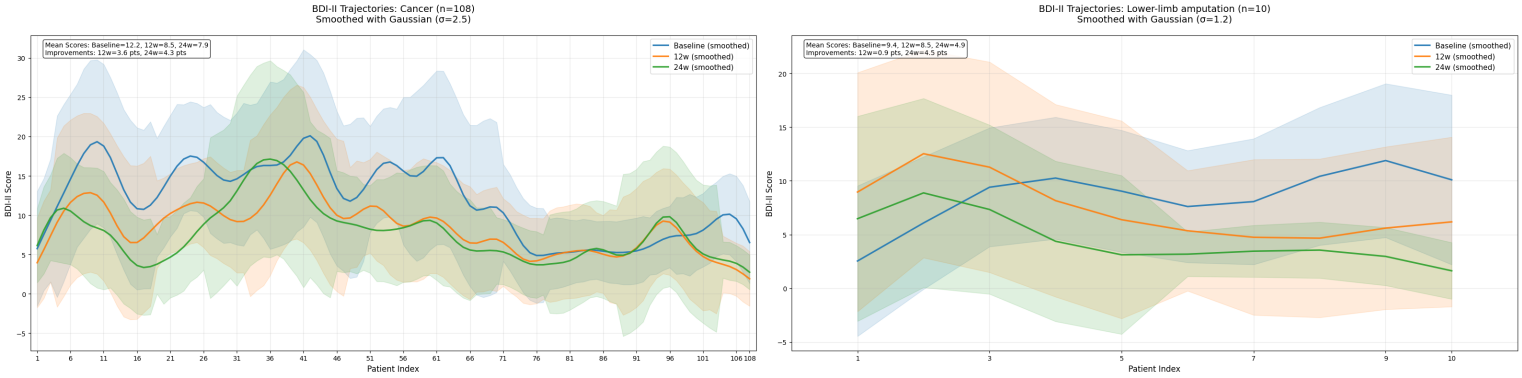
\includegraphics[width=0.48\linewidth]{temp1.png}
    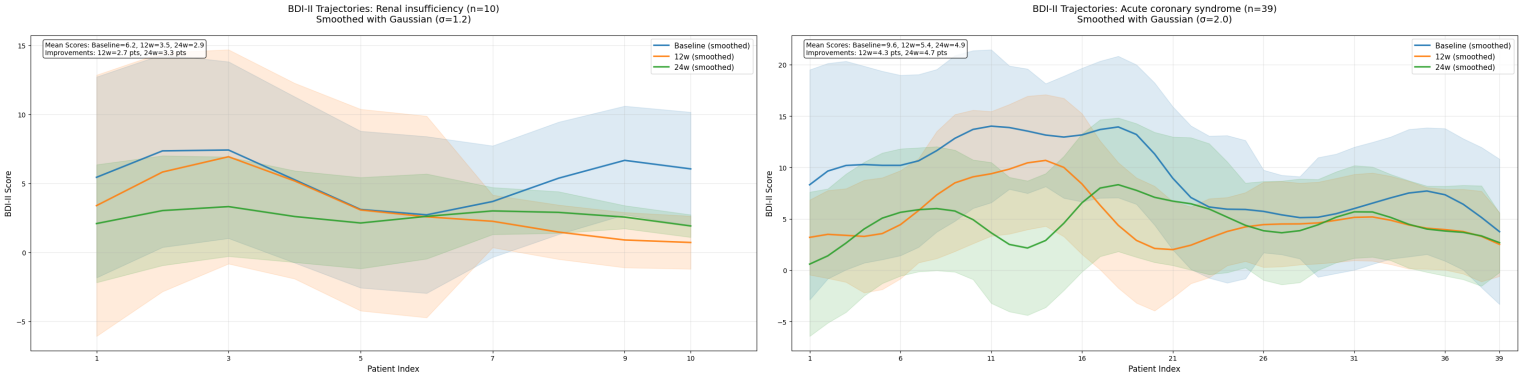
\includegraphics[width=0.48\linewidth]{temp2.png}
    \caption{Comparison of BDI-II scores at baseline, 12-week, and 24-week follow-up, visualizing the score trends for all types of conditions (Cancer, Lower-Limb Amputation, Renal Insufficiency, Acute Coronary Syndrome).}
    \label{fig:bdi_distri_hospital}
\end{figure*}

Four primary medical conditions and seven subtypes were one-hot encoded. BDI-II baseline scores were log-transformed, squared, and categorized for continuous and categorical measures. Age was segmented (young, middle, mature, senior) and scaled nonlinearly via age squared, noting many patients $>45$. Mindfulness engagement was quantified through completion rates and adherence levels (low, medium, high), and sex was binary encoded. Disease burden metrics included total conditions and unique subtypes per patient. Analysis showed patients with lower-limb amputation and renal insufficiency had the highest 12-week success rates (63.9\% and 61.1\%), while cancer and acute coronary syndrome had lower initial rates that declined by 24 weeks. Higher completion improved outcomes for cancer and acute coronary syndrome, but lower completion corresponded to greater improvement for lower-limb amputations.




\begin{table}[ht]
\centering
\caption{Mean BDI-II score improvements from baseline at 12- and 24-week follow-ups across different medical condition types.}
\begin{tabularx}{\linewidth}{|X|c|c|}
\hline
\textbf{Condition Type} & \textbf{12 Week Improvement} & \textbf{24 Week Improvement} \\
\hline
Breast & 4.76 & 5.73 \\ 
Dialysis & 10.00 & 9.00 \\ 
No prosthesis & 0.30 & 4.50 \\ 
Percutaneous CT & 2.25 & 2.125 \\ 
Predialysis & 1.88 & 2.66 \\ 
Prostate & 1.83 & 1.93 \\ 
Revascularization & 4.77 & 5.00 \\ 
\hline
\end{tabularx}
\label{tab:bdii_improvement}
\end{table}


The dataset included 26 numeric features and two targets, with all categorical and clinical variables standardized for machine learning. Features were grouped as: Demographics (age, sex), Clinical Baseline (baseline BDI-II), Medical Comorbidities (Cancer, ACS, Renal, LLA~\footnote{Acute Coronary Syndrome (ACS) and Lower-Limb Amputation (LLA) are abbreviated as shown.} ; see Table~\ref{tab:bdii_improvement} for 12- and 24-week improvements) , Treatment Engagement (session completion, mindfulness; average 71.81\%), and Prediction Targets (BDI-II at 12 and 24 weeks). Patients with higher baseline BDI-II scores showed greater improvements (Table~\ref{tab:severity_metrics_mean}). Patients in the severe category, who received the most intensive engagement, had the highest improvements of 16.2 and 17.8.


\begin{table}
\centering
\caption{Baseline Severity and Improvement Metrics (Mean Values)}
\label{tab:severity_metrics_mean}
\begin{tabularx}{\linewidth}{|X|X|X|X|X|}
\hline
\textbf{Baseline Severity} & \textbf{Completion Rate} & \textbf{12w Improvement} & \textbf{24w Improvement} & \textbf{BDI-II Baseline} \\
\hline
Minimal & 0.721 & 1.239 & 1.632 & 6.639 \\ 
Mild & 0.707 & 6.250 & 8.071 & 16.353 \\ 
Moderate & 0.704 & 10.800 & 11.857 & 23.348 \\ 
Severe& 0.762 & 16.286 & 17.857 & 35.625 \\
\hline
\end{tabularx}
\end{table}

% \begin{figure}
%     \centering
%     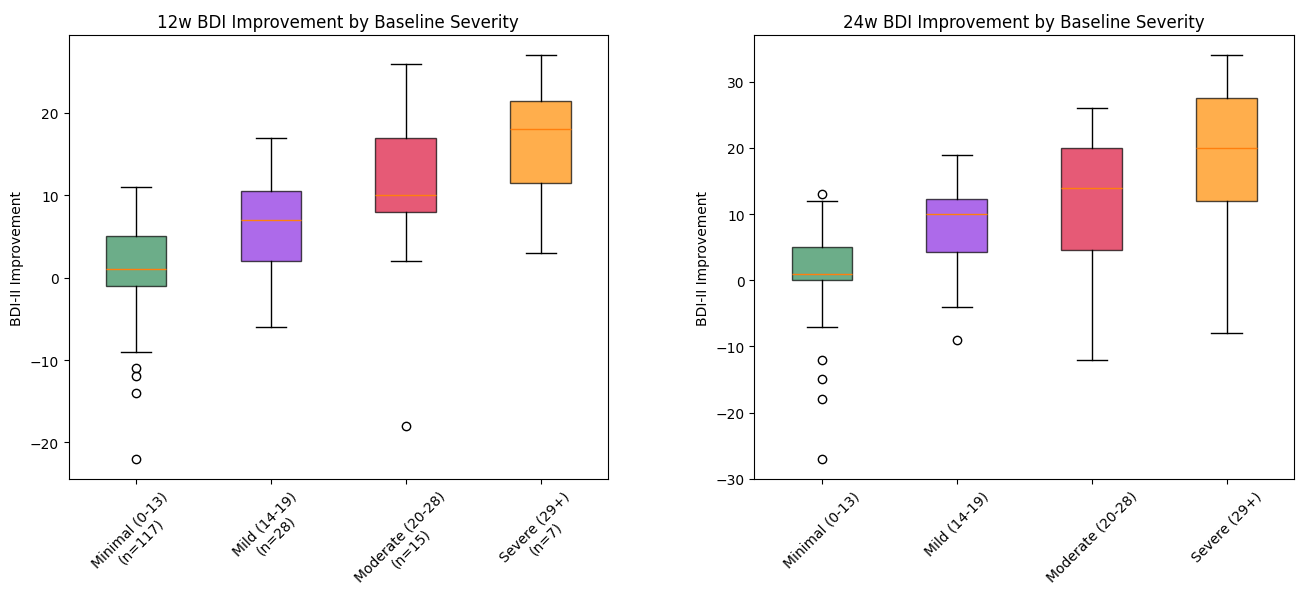
\includegraphics[width=1\linewidth]{bdi_distri_severity.png}
%     \caption{Baseline Severity and Improvement Metrics}
%     \label{tab:severity_metrics_mean}
% \end{figure}



% ----
\section{Planned Methodology}

Our primary objective was to develop robust predictive models to estimate patient's BDI-II scores at 12-week and 24-week follow-ups. To achieve this, we framed the challenge as two independent supervised regression tasks using a rigorous multi-phase models experimentation.
\subsection{Multi-Phase Modeling Strategy}
We implement a systematic five-phase experimental framework designed to comprehensively explore the model complexity spectrum while maintaining interpretability and clinical relevance (Table~\ref{tab:phases}). Linear models provide interpretability and feature importance. Classical ML methods capture non-linear relationships. Ensembles combine multiple perspectives for improved performance. Deep learning explores MLPs, attention, and ResNet-based architectures. Time-series models (LSTM, GRU, Transformer) leverage longitudinal patient data.

\begin{table}[h]
\centering
\caption{Multi-Phase Modeling Framework}
\label{tab:phases}
\resizebox{\columnwidth}{!}{%
\begin{tabular}{@{}llll@{}}
\toprule
\textbf{Phase} & \textbf{Category} & \textbf{Key Models} & \textbf{\# Models} \\ \midrule
1 & Linear Baselines & Lasso, Ridge, ElasticNet, Bayesian Ridge, etc & 8 \\
2 & Classical ML & Random Forest, SVR variants, KNN, GB, etc & 10 \\
3 & Ensembles & XGBoost, CatBoost, Stacking, Voting, etc & 5 \\
4 & Deep Learning & MLP variants, Attention, ResNet, etc & 7 \\
5 & Time-series & Transformer, LSTM, GRU, Trajectory, etc & 10 \\ \midrule
\multicolumn{3}{l}{\textbf{Total Models Evaluated}} & \textbf{40} \\ \bottomrule
\end{tabular}%
}
\end{table}


\begin{table*}[h!]
\centering
\caption{Model performance metrics at 12- and 24-week follow-ups. The table presents comprehensive results across all five model phases, with the top-performing models highlighted: Top 1 in red, Top 2 in purple, and Top 3 in blue for both 12- and 24-week evaluations. Models within each phase are grouped by cell color, and phases are arranged sequentially from Phase 1 (top-left) to Phase 5 (bottom-right).}
\label{tab:model_performance_phases}
\resizebox{\linewidth}{!}{
\begin{tabular}{@{}lrrrr@{\hspace{0.8em}}|@{\hspace{0.8em}}lrrrr@{}}
\toprule
\textbf{Model} & \textbf{12-Wk $R^2$} & \textbf{12-Wk MAE} & \textbf{24-Wk $R^2$} & \textbf{24-Wk MAE} & \textbf{Model} & \textbf{12-Wk $R^2$} & \textbf{12-Wk MAE} & \textbf{24-Wk $R^2$} & \textbf{24-Wk MAE} \\
\midrule
% Phase 1 (Left) | Phase 3 (Right)
\cellcolor{phase1color}Linear Regression & \cellcolor{phase1color}$-0.03 \pm 0.24$ & \cellcolor{phase1color}$5.18 \pm 0.34$ & \cellcolor{phase1color}$-0.02 \pm 0.25$ & \cellcolor{phase1color}$5.08 \pm 0.65$ & \cellcolor{phase3color}Voting Regressor & \cellcolor{phase3color}$-0.17 \pm 0.35$ & \cellcolor{phase3color}$5.39 \pm 0.55$ & \cellcolor{phase3color}$0.09 \pm 0.30$ & \cellcolor{phase3color}$4.70 \pm 0.42$ \\ \vspace{1pt}
\cellcolor{phase1color}Ridge Regression & \cellcolor{phase1color}$0.15 \pm 0.17$ & \cellcolor{phase1color}$4.79 \pm 0.38$ & \cellcolor{phase1color}$0.09 \pm 0.21$ & \cellcolor{phase1color}$4.73 \pm 0.38$ & \cellcolor{phase3color}Stacking Regressor & \cellcolor{phase3color}$0.07 \pm 0.12$ & \cellcolor{phase3color}$5.18 \pm 0.72$ & \cellcolor{phase3color}$0.11 \pm 0.19$ & \cellcolor{phase3color}$4.80 \pm 0.48$ \\ \vspace{1pt} 
\cellcolor{phase1color}\color{purple}{\textbf{Lasso Regression}} & \cellcolor{phase1color}\color{purple}{\textbf{$0.18 \pm 0.11$}} & \cellcolor{phase1color}\color{purple}{\textbf{$4.71 \pm 0.53$}} & \cellcolor{phase1color}$0.09 \pm 0.18$ & \cellcolor{phase1color}$4.68 \pm 0.43$ & \cellcolor{phase3color}Advanced Stacking & \cellcolor{phase3color}$0.04 \pm 0.16$ & \cellcolor{phase3color}$5.26 \pm 0.66$ & \cellcolor{phase3color}$0.13 \pm 0.18$ & \cellcolor{phase3color}$4.77 \pm 0.46$ \\ \vspace{1pt}
% Phase 1 (Left) | Phase 4 (Right)
\cellcolor{phase1color}\color{blue}{\textbf{Elastic Net}} & \cellcolor{phase1color}\color{blue}{\textbf{$0.16 \pm 0.16$}} & \cellcolor{phase1color}\color{blue}{\textbf{$4.77 \pm 0.43$}} & \cellcolor{phase1color}$0.09 \pm 0.19$ & \cellcolor{phase1color}$4.68 \pm 0.41$ & \cellcolor{phase4color}MLP (Small) & \cellcolor{phase4color}$0.05 \pm 0.09$ & \cellcolor{phase4color}$5.24 \pm 0.65$ & \cellcolor{phase4color}$0.06 \pm 0.14$ & \cellcolor{phase4color}$4.88 \pm 0.08$ \\ \vspace{1pt}
\cellcolor{phase1color}Bayesian Ridge & \cellcolor{phase1color}$0.14 \pm 0.17$ & \cellcolor{phase1color}$4.79 \pm 0.36$ & \cellcolor{phase1color}$0.08 \pm 0.21$ & \cellcolor{phase1color}$4.74 \pm 0.39$ & \cellcolor{phase4color}MLP (Medium) & \cellcolor{phase4color}$0.13 \pm 0.13$ & \cellcolor{phase4color}$4.96 \pm 0.31$ & \cellcolor{phase4color}$0.15 \pm 0.15$ & \cellcolor{phase4color}$4.73 \pm 0.17$ \\ \vspace{1pt}
\cellcolor{phase1color}Huber Regressor & \cellcolor{phase1color}$0.11 \pm 0.16$ & \cellcolor{phase1color}$4.79 \pm 0.49$ & \cellcolor{phase1color}$0.02 \pm 0.20$ & \cellcolor{phase1color}$4.68 \pm 0.21$ & \cellcolor{phase4color}\color{purple}{\textbf{MLP (Large)}} & \cellcolor{phase4color}$-0.04\pm0.18$ & \cellcolor{phase4color}$5.30\pm0.98$ & \cellcolor{phase4color}\color{purple}{\textbf{$0.16\pm0.13$ }}& \cellcolor{phase4color}\color{purple}{\textbf{$4.64\pm0.09$}} \\ \vspace{1pt}
\cellcolor{phase1color}RANSAC Regressor & \cellcolor{phase1color}$-0.37 \pm 0.39$ & \cellcolor{phase1color}$5.98 \pm 1.05$ & \cellcolor{phase1color}$-0.96 \pm 0.76$ & \cellcolor{phase1color}$6.80 \pm 1.49$ & \cellcolor{phase4color}TF MLP (Simple) & \cellcolor{phase4color}$-0.12 \pm 0.16$ & \cellcolor{phase4color}$5.29 \pm 0.85$ & \cellcolor{phase4color}$0.04 \pm 0.06$ & \cellcolor{phase4color}$4.66 \pm 0.12$ \\ \vspace{1pt}
\cellcolor{phase1color}Decision Tree & \cellcolor{phase1color}$-0.07 \pm 0.14$ & \cellcolor{phase1color}$5.19 \pm 0.64$ & \cellcolor{phase1color}$-0.06 \pm 0.40$ & \cellcolor{phase1color}$4.81 \pm 0.63$ & \cellcolor{phase4color}TF MLP (Deep) & \cellcolor{phase4color}$-0.35 \pm 0.70$ & \cellcolor{phase4color}$5.53 \pm 1.27$ & \cellcolor{phase4color}$-0.31 \pm 0.32$ & \cellcolor{phase4color}$5.49 \pm 0.93$ \\ \vspace{1pt}
% Phase 2 (Left) | Phase 4 (Right)
\cellcolor{phase2color}Random Forest & \cellcolor{phase2color}$0.09 \pm 0.19$ & \cellcolor{phase2color}$4.82 \pm 0.45$ & \cellcolor{phase2color}$0.14 \pm 0.25$ & \cellcolor{phase2color}$4.52 \pm 0.44$ & \cellcolor{phase4color}TF ResNet & \cellcolor{phase4color}$0.05 \pm 0.11$ & \cellcolor{phase4color}$4.83 \pm 0.66$ & \cellcolor{phase4color}$-0.31 \pm 0.27$ & \cellcolor{phase4color}$5.31 \pm 0.72$ \\ \vspace{1pt}
\cellcolor{phase2color}Extra Trees & \cellcolor{phase2color}$0.05 \pm 0.25$ & \cellcolor{phase2color}$4.93 \pm 0.36$ & \cellcolor{phase2color}$-0.01 \pm 0.39$ & \cellcolor{phase2color}$4.78 \pm 0.38$ & \cellcolor{phase4color}TF Attention & \cellcolor{phase4color}$0.15 \pm 0.07$ & \cellcolor{phase4color}$4.78 \pm 0.34$ & \cellcolor{phase4color}$0.12 \pm 0.07$ & \cellcolor{phase4color}$4.62 \pm 0.08$ \\ \vspace{1pt}
% Phase 2 (Left) | Phase 5 (Right)
\cellcolor{phase2color}AdaBoost & \cellcolor{phase2color}$0.09 \pm 0.15$ & \cellcolor{phase2color}$4.83 \pm 0.53$ & \cellcolor{phase2color}$0.11 \pm 0.23$ & \cellcolor{phase2color}$4.65 \pm 0.53$ & \cellcolor{phase5color}ARIMA & \cellcolor{phase5color}$-0.21 \pm 0.21$ & \cellcolor{phase5color}$5.71 \pm 0.97$ & \cellcolor{phase5color}$-0.23 \pm 0.25$ & \cellcolor{phase5color}$5.14 \pm 1.27$ \\ \vspace{1pt}
\cellcolor{phase2color}Gradient Boosting & \cellcolor{phase2color}$0.06 \pm 0.19$ & \cellcolor{phase2color}$5.07 \pm 0.48$ & \cellcolor{phase2color}$0.03 \pm 0.26$ & \cellcolor{phase2color}$4.79 \pm 0.54$ & \cellcolor{phase5color}Exponential Smoothing & \cellcolor{phase5color}$-0.20 \pm 0.06$ & \cellcolor{phase5color}$5.87 \pm 0.83$ & \cellcolor{phase5color}$-0.29 \pm 0.38$ & \cellcolor{phase5color}$5.31 \pm 1.53$ \\ \vspace{1pt}
\cellcolor{phase2color}SVR (Linear) & \cellcolor{phase2color}$0.14 \pm 0.12$ & \cellcolor{phase2color}$4.67 \pm 0.58$ & \cellcolor{phase2color}$0.03 \pm 0.15$ & \cellcolor{phase2color}$4.56 \pm 0.26$ & \cellcolor{phase5color}Moving Average & \cellcolor{phase5color}$-0.50 \pm 0.35$ & \cellcolor{phase5color}$6.38 \pm 1.08$ & \cellcolor{phase5color}$-0.40 \pm 0.23$ & \cellcolor{phase5color}$5.80 \pm 1.39$ \\ \vspace{1pt}
\cellcolor{phase2color}SVR (RBF) & \cellcolor{phase2color}$0.15 \pm 0.08$ & \cellcolor{phase2color}$4.73 \pm 0.81$ & \cellcolor{phase2color}$0.11 \pm 0.18$ & \cellcolor{phase2color}$4.49 \pm 0.34$ & \cellcolor{phase5color}LSTM (Simple) & \cellcolor{phase5color}$0.05 \pm 0.06$ & \cellcolor{phase5color}$5.33 \pm 0.48$ & \cellcolor{phase5color}$0.01 \pm 0.03$ & \cellcolor{phase5color}$5.08 \pm 0.34$ \\ \vspace{1pt}
\cellcolor{phase2color}SVR (Poly) & \cellcolor{phase2color}$0.04 \pm 0.22$ & \cellcolor{phase2color}$5.24 \pm 1.06$ & \cellcolor{phase2color}$-0.01 \pm 0.10$ & \cellcolor{phase2color}$4.80 \pm 0.69$ & \cellcolor{phase5color}LSTM (Bi-dir) & \cellcolor{phase5color}$0.13 \pm 0.07$ & \cellcolor{phase5color}$5.13 \pm 0.57$ & \cellcolor{phase5color}$-0.01 \pm 0.03$ & \cellcolor{phase5color}$5.19 \pm 0.34$ \\ \vspace{1pt}
\cellcolor{phase2color}NU SVR & \cellcolor{phase2color}$0.14 \pm 0.07$ & \cellcolor{phase2color}$4.74 \pm 0.91$ & \cellcolor{phase2color}$0.05 \pm 0.10$ & \cellcolor{phase2color}$4.51 \pm 0.56$ & \cellcolor{phase5color}LSTM (Stacked) & \cellcolor{phase5color}$0.13 \pm 0.12$ & \cellcolor{phase5color}$5.03 \pm 0.61$ & \cellcolor{phase5color}$-0.01 \pm 0.01$ & \cellcolor{phase5color}$5.11 \pm 0.37$ \\ \vspace{1pt}
\cellcolor{phase2color}KNN Regressor & \cellcolor{phase2color}$0.13 \pm 0.14$ & \cellcolor{phase2color}$5.01 \pm 0.57$ & \cellcolor{phase2color}$0.12 \pm 0.19$ & \cellcolor{phase2color}$4.55 \pm 0.56$ & \cellcolor{phase5color}GRU & \cellcolor{phase5color}$0.08 \pm 0.05$ & \cellcolor{phase5color}$5.22 \pm 0.47$ & \cellcolor{phase5color}$0.01 \pm 0.04$ & \cellcolor{phase5color}$5.18 \pm 0.37$ \\ \vspace{1pt}
\cellcolor{phase2color}KNN Uniform & \cellcolor{phase2color}$0.15 \pm 0.14$ & \cellcolor{phase2color}$4.95 \pm 0.64$ & \cellcolor{phase2color}$0.01 \pm 0.22$ & \cellcolor{phase2color}$4.62 \pm 0.67$ & \cellcolor{phase5color}\color{red}{\textbf{Transformer}} & \cellcolor{phase5color}\color{red}{\textbf{$0.24\pm0.09$}} & \cellcolor{phase5color}\color{red}{\textbf{$4.53\pm0.56$}} & \cellcolor{phase5color}$0.08\pm0.14$ & \cellcolor{phase5color}$4.97\pm0.61$ \\ \vspace{1pt}
% Phase 3 (Left) | Phase 5 (Right)
\cellcolor{phase3color}XGBoost & \cellcolor{phase3color}$0.09 \pm 0.14$ & \cellcolor{phase3color}$5.00 \pm 0.63$ & \cellcolor{phase3color}$0.13 \pm 0.24$ & \cellcolor{phase3color}$4.63 \pm 0.55$ & \cellcolor{phase5color}\color{blue}{\textbf{RF Trajectory}} & \cellcolor{phase5color}$0.01 \pm 0.20$ & \cellcolor{phase5color}$5.12 \pm 0.02$ & \cellcolor{phase5color}\color{blue}{\textbf{$0.16 \pm 0.12$}} & \cellcolor{phase5color}\color{blue}{\textbf{$4.80 \pm 0.28$}} \\ \vspace{1pt}
\cellcolor{phase3color}\color{red}{\textbf{Catboost}} & \cellcolor{phase3color}$0.09\pm0.16$ & \cellcolor{phase3color}$4.91\pm0.51$ & \cellcolor{phase3color}\color{red}{\textbf{$0.20\pm0.13$}} & \cellcolor{phase3color}\color{red}{\textbf{$4.36\pm0.58$}} & \cellcolor{phase5color}Ridge Trajectory & \cellcolor{phase5color}$0.07 \pm 0.15$ & \cellcolor{phase5color}$4.99 \pm 0.23$ & \cellcolor{phase5color}$0.10 \pm 0.15$ & \cellcolor{phase5color}$4.95 \pm 0.38$ \\
\bottomrule
\end{tabular}
}
\end{table*}


\subsection{Experimental Setup}
We trained the same set of 26 engineered features across 40 models for both 12- and 24-week BDI-II prediction tasks to ensure a consistent and fair comparison. Each model underwent systematic hyperparameter tuning using Bayesian Optimization, which efficiently explores complex parameter spaces to minimize prediction error. The best-performing model from each task was selected for in-depth analysis, with detailed performance results provided in Table~\ref{tab:model_performance_phases}. Experiments were conducted on an Acer Nitro 5 laptop with an \textbf{Intel i7-12650H} processor (16 CPUs, $\thickapprox$2.7GHz) and 16GB RAM. This setup allowed rigorous evaluation while balancing computational efficiency.


\subsection{Evaluation Framework}

Model performance is assessed through rigorous 5-fold cross-validation with stratification to maintain consistent target distribution across folds. Test set performance determined final rankings. Primary metrics were:

\noindent \textbf{R² Score:} Proportion of variance explained by the model:
\[
R^2 = 1 - \frac{\sum_{i=1}^{n} (y_i - \hat{y}_i)^2}{\sum_{i=1}^{n} (y_i - \bar{y})^2}
\]
where $y_i$ and $\hat{y}_i$ are actual and predicted values, $\bar{y}$ is the mean of $y_i$, and $n$ is the number of samples.

\noindent \textbf{Mean Absolute Error (MAE):} Average magnitude of prediction errors:
\[
\text{MAE} = \frac{1}{n} \sum_{i=1}^{n} |y_i - \hat{y}_i|
\]
where $y_i$ and $\hat{y}_i$ are actual and predicted values. Lower MAE indicates better accuracy.

The other metrics we have considered are RMSE, MAPE, but as of the time being we would completely depend on the above two metrics mentioned.

\subsection{Interpretability and Clinical Insights}

Model interpretability was assessed via SHAP to obtain global and instance-level feature importance. Disease-specific subgroup analyses were conducted to evaluate differential performance across primary conditions, with statistical significance tested.

\section{Results}

A total of 40 models, including classical ML and simple deep learning, were evaluated for predicting BDI-II scores at 12- and 24-week follow-ups. Cross-validated mean and standard deviation of R² and MAE are summarized in Table~\ref{tab:model_performance_phases}. An R² of 0.2 is generally considered acceptable, 0.3–0.5 is strong, and values above 0.5 are rare in real-world mental health studies~\cite{b6,b7,b8}.

For the 12-week prediction, deep learning models performed best, with the Transformer model as the top performer, followed by Lasso Regression and Elastic Net. For the 24-week task, CatBoost led, followed by MLP Large and RF Trajectory models. Figure~\ref{fig:hyper_param_tuned} shows the hyperparameter tuning heatmaps for both top models. These two models were selected for further analysis.


\begin{figure}[th]
    \centering
    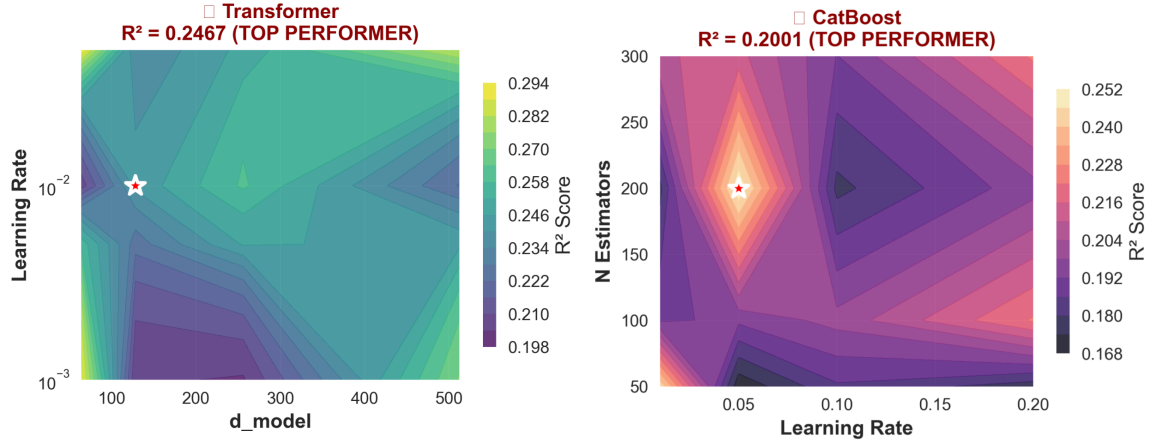
\includegraphics[width=1\linewidth]{hyper-parameter-comp.png}
    \caption{Hyperparameter tuning heatmaps for the top-performing models: Transformer (left) and CatBoost (right). The plots visualize the performance (R² score) across different hyperparameter values. The white star pinpoints the optimal combination that yielded the highest R² score for each model.}
    \label{fig:hyper_param_tuned}
\end{figure}

\section{Feature Importance Insights}
The Baseline BDI-II score dominates with it's ~40\% of explained variance, followed by ~15\% contribution by age, 12\% contribution by Treatment Engagement (therapy completion rate, attendance etc) and ~15\% by all medical indicator combined, as seen in Figure~\ref{fig:shap_global}. These results strongly suggests that patients with higher baseline BDI-II score exhibit greater score at follow-up, while the older patients improve slower, suggesting age-based treatment and also higher treatment engagment results in improved outcomes. From 12- to 24-week follow-up, Demographic features slightly decreased to 90\%, Clinical remained stable, while Therapy and Condition features rose sharply to 296\% and 111\%, respectively, highlighting the importance of therapy sessions (mindfullness) for the long run.

We observed that 62.3\% of patients responded to mindfulness, 14.4\% improved only by 24 weeks (late responders), 8.4\% relapsed after an initial response (early responders), and 15\% showed no improvement (no response). Responders improved on average by $4.99 \pm 6.47$ at 12 weeks and $5.38 \pm 7.27$ at 24 weeks. Early responders had strong 12-week gains ($8.36 \pm 6.69$) but plateaued by 24 weeks, while late responders improved mainly at 24 weeks ($8.29 \pm 6.71$), reflecting the impact of treatment engagement timing.


\begin{figure}[t]
\centering
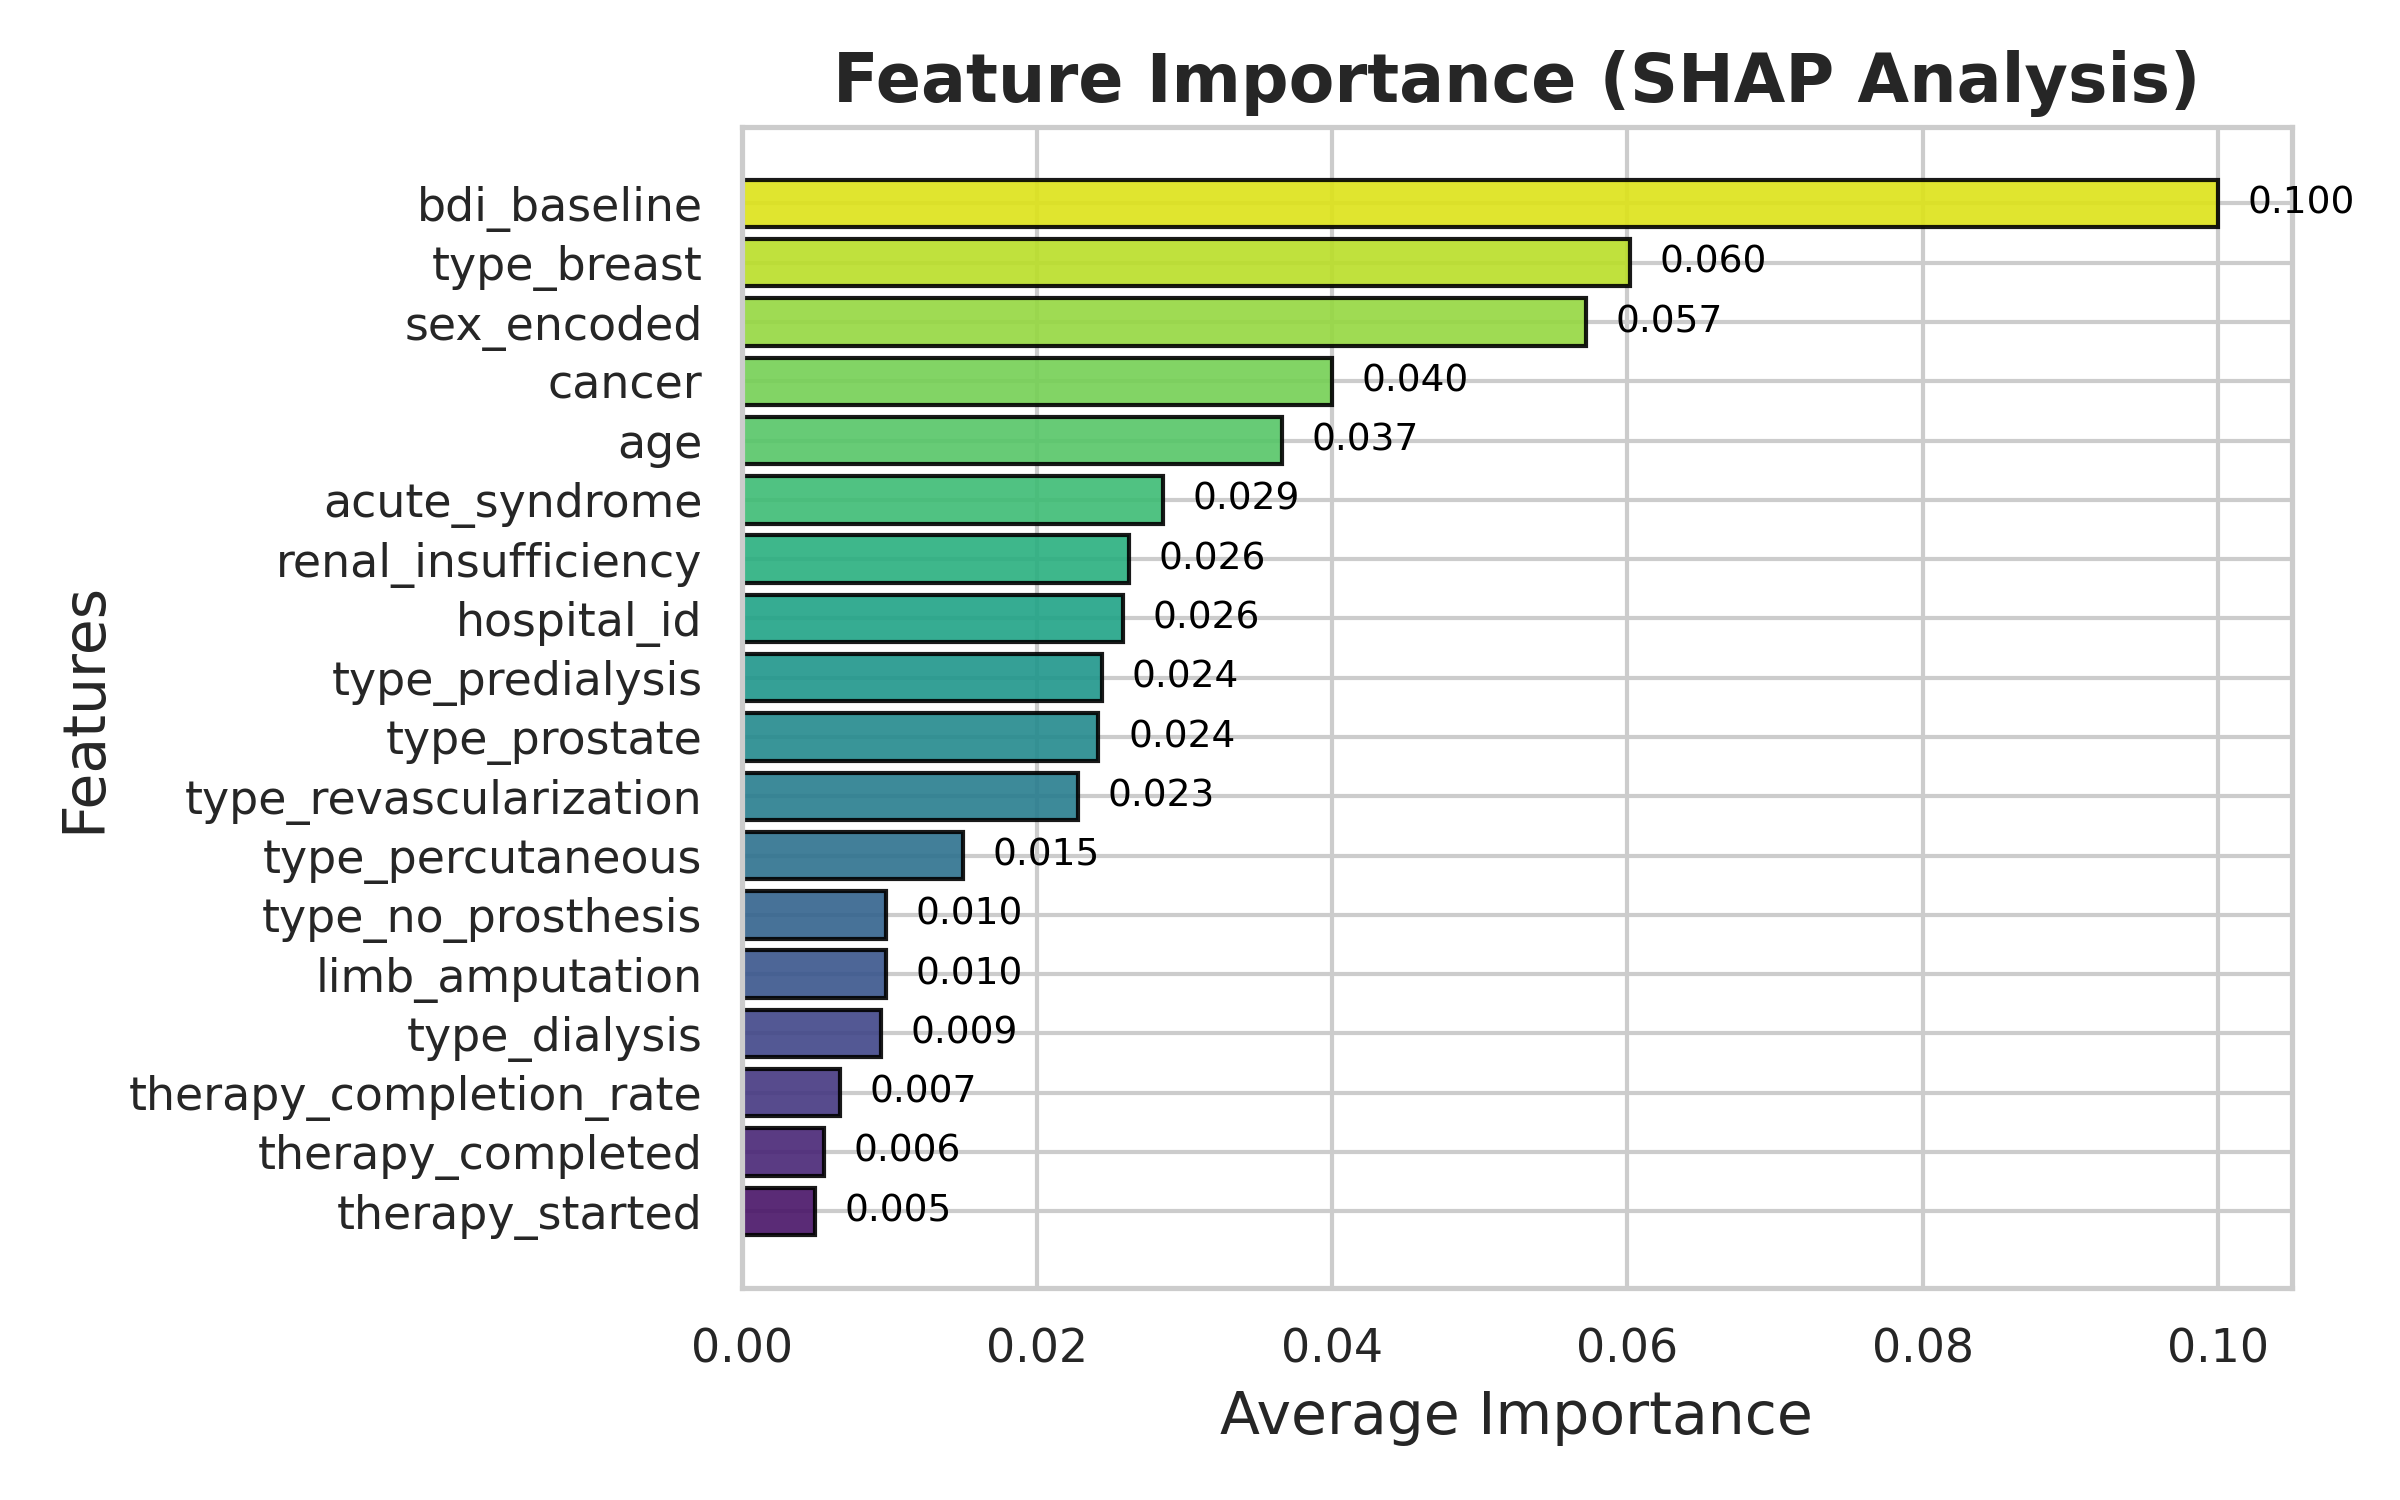
\includegraphics[width=0.48\textwidth]{feature_importance.png}
\caption{Global SHAP feature importance across best-performing models. Baseline BDI-II score dominates, followed by age and treatment engagement metrics.}
\label{fig:shap_global}
\end{figure}


\section{Disease-Specific Analysis}

The most significant finding of our study is the profound impact of a patient's primary medical diagnosis on their depression treatment outcome. As illustrated by the distinct patient pathways in Figure \ref{fig:disease_specific_analysis}, different clinical cohorts respond to the mindfulness intervention in fundamentally different ways. This clinical heterogeneity is so pronounced that when we trained models on specific disease subgroups, predictive accuracy skyrocketed from a general population R² of 0.247 to R² scores exceeding 0.90 (Table \ref{tab:condition_performance}), confirming that a disease-specific analytical framework is essential.


\begin{figure}[th]
    \centering
    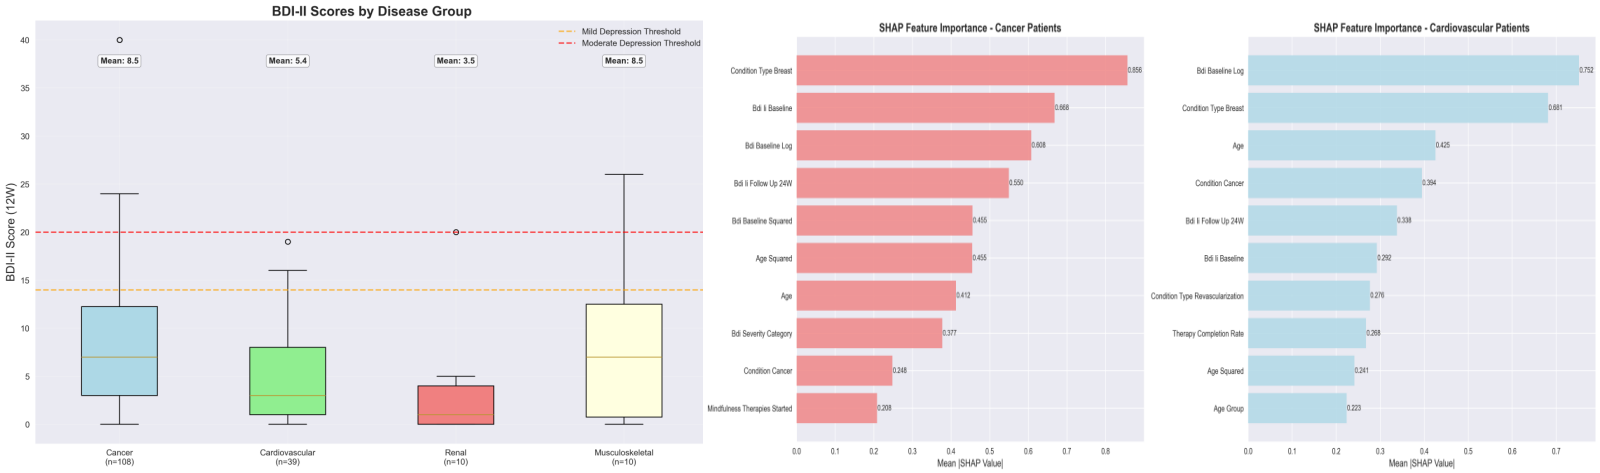
\includegraphics[width=1\linewidth]{disease_specific_analysis.png}
    \caption{Longitudinal BDI-II score trajectories for individual patients, stratified by the four primary medical cohorts. The plots visualize patient progress from baseline to the 12-week and 24-week follow-ups.}
    \label{fig:disease_specific_analysis}
\end{figure}


\textbf{Cancer Patients} (64.7\%, n=108) constitute the largest subgroup and exhibit significantly elevated depression scores. At 12-week follow-up, cancer patients average BDI = 8.51 ± 7.68 compared to 5.59 ± 6.07 for non-cancer patients (difference = +2.92, p = 0.007, Cohen's d = 0.41). This moderate-to-large effect size persists at 24 weeks (difference = +3.31, p = 0.001, d = 0.46), indicating that cancer-related psychological burden remains substantial despite mindfulness intervention. The consistent effect suggests need for cancer-specific augmented interventions.

\textbf{Renal Insufficiency} (6.0\%, n=10) demonstrates an unexpected protective pattern. Patients with renal conditions show mean BDI = 3.50 ± 6.13 versus 7.73 ± 7.28 for those without (difference = -4.23, p = 0.017, d = -0.59). While the small sample size warrants cautious interpretation, the statistically significant moderate effect persists at 24 weeks (p = 0.046), suggesting genuine protective factors potentially including close medical monitoring, structured treatment adherence, or resilience developed through chronic disease management.

\textbf{Acute Coronary Syndrome} (23.4\%, n=39) shows non-significant trends toward lower depression at 12 weeks (mean = 5.38 vs. 8.12, p = 0.071), reaching significance by 24 weeks (p = 0.044, d = -0.32). This delayed effect may reflect gradual cardiovascular rehabilitation benefits or reduced acute medical stress.

\textbf{Lower limb amputation} (6.0\%, n=10) demonstrates neutral effects: mean BDI = 8.50 vs. 7.41 (non-amputation), difference = +1.09, p = 0.884, d = 0.15. The small non-significant effect indicates amputation status alone does not substantially predict depression outcomes. At 24W, a trend toward improvement emerges (difference = -1.93, p = 0.351), though remains non-significant, suggesting adaptation or prosthetic rehabilitation benefits may require longer observation.




\begin{table}
\centering
\caption{Prediction Performance by Condition Group}
\label{tab:condition_performance}
\begin{tabularx}{\linewidth}{XXXXX}
\hline
\textbf{Disease Group} & \textbf{R\textsuperscript{2} Score} & \textbf{Mean Prediction} & \textbf{Mean Actual} & \textbf{Feature Imp}\\
\midrule
Cancer & 0.928 & $8.42\pm6.46$ & $8.51\pm7.65$ & 39.8\%  \\
Acute Cor. & 0.812 & $5.72\pm3.51$ & $5.38\pm5.05$ & 26.8\% \\
Renal & 0.922 & $3.86\pm4.49$ & $3.50\pm5.82$ & 19.2\% \\
Lower Li. & 0.888 & $8.31\pm6.82$ & $8.50\pm8.22$ & 14.2\% \\
\bottomrule
\end{tabularx}
\end{table}

\subsection{Therapy Engagement by Medical Condition}

Therapy engagement exhibits condition-specific patterns with differential impacts on outcomes (Table~\ref{tab:therapy_engagement}). Only cancer patients demonstrate highest engagement rate (72.2\%), compared to non-cancer (49.9\%) and benefit 24 week therapy-BDI negative correlation with 4.19 lower BDI scores. In contrast, ACS patients show lowest engagement (49.1\%) and paradoxical positive correlations at 24 week, suggesting reverse causation where more symptomatic individuals engage more. Renal patients show a similar pattern as ACS, despite low baseline BDI (3.5), implying protective medical factors. Amputation patients show similar patterns, without a significant therapy-BDI relation, indicating that physical rehabilitation supersedes mindfulness benefit. Overall, these results advocate condition-stratified interventions—enhancing therapy access for cancer patients while tailoring alternatives for other conditions.

\begin{table}[h]
\centering
\caption{Therapy Engagement and Depression Outcomes by Medical Condition}
\parbox[t]{\linewidth}{\vspace{1ex}\footnotesize
Comp. Rate = therapy completion rate; Engage. vs Non = difference from patients without condition; 
$r$ = Pearson correlation (Spearman for ACS 24W); Effect (Hi–Lo) = BDI difference between high vs low engagement groups at 24W; }
\label{tab:therapy_engagement}
\resizebox{\columnwidth}{!}{%
\begin{tabular}{@{}lcccccc@{}}
\toprule
\textbf{Condition} & 
\makecell[c]{\textbf{Comp.}\\\textbf{Rate}} & 
\makecell[c]{\textbf{Engage.}\\\textbf{vs Non}} & 
\makecell[c]{\textbf{r\textsubscript{12W}}\\\textbf{(BDI)}} & 
\makecell[c]{\textbf{r\textsubscript{24W}}\\\textbf{(BDI)}} & 
\makecell[c]{\textbf{p\textsubscript{24W}}} & 
\makecell[c]{\textbf{Effect}\\\textbf{(Hi–Lo)}} \\
\midrule
Cancer & 77.2\% & +27.4\% & -0.133 & \textbf{-0.232} & \textbf{0.016} & \textbf{-4.19*} \\
ACS & 49.1\% & -24.0\% & -0.114 & \textbf{+0.374} & \textbf{0.019} & \textbf{+2.83*} \\
Renal & 58.7\% & -9.1\% & +0.466 & \textbf{+0.656} & \textbf{0.039} & +3.40 \\
Amputation & 43.8\% & -25.3\% & +0.354 & +0.333 & 0.346 & +3.80 \\
\bottomrule
\end{tabular}%
}
\end{table}

\section{Conclusion}

This preliminary analysis establishes a rigorous multi-phase modeling framework for predicting depression outcomes following mindfulness-based interventions. Our systematic evaluation of 38 models across five methodological phases reveals that timepoint-specific architectures—Transformer for 12-week and CatBoost for 24-week predictions—achieve optimal performance with test R² scores of 0.247 and 0.200, respectively. Disease-specific analysis uncovers significant condition-dependent effects, particularly the elevated depression burden in cancer patients and unexpected protective patterns in renal insufficiency cohorts. SHAP-based interpretability analysis identifies baseline severity, age, and treatment engagement as primary predictive drivers while revealing complex medical comorbidity interactions. These early findings provide a strong foundation for developing clinically deployable, interpretable prediction systems that can support personalized treatment planning and risk stratification in depression care. Ongoing work focuses on ensemble integration, trajectory phenotyping, and external validation to translate these preliminary results into robust clinical decision support tools.

\section{New Conclusion}

This mid-term study demonstrates that machine learning effectively predicts depression trajectories in medically complex populations undergoing mindfulness interventions. Systematic evaluation of 40 models across five phases reveals timepoint-specific optimal architectures: Transformer for 12-week (R² = 0.247, MAE = 4.53) and CatBoost for 24-week predictions (R² = 0.200, MAE = 4.36).

\textbf{Key Clinical Findings:} Medical condition profoundly impacts treatment response. Cancer patients (64.7\%) show elevated depression (+2.92–3.31 BDI points, p < 0.01) but strongest therapy benefits (77.2\% completion; high-engagement achieves 4.19-point greater reduction, r = -0.232, p = 0.016). Renal patients display unexpected resilience (4.23 points lower, p = 0.017). ACS patients exhibit paradoxical reverse causation (ρ = +0.374, p = 0.019). Disease-stratified models achieve exceptional accuracy (R² = 0.81–0.93), confirming condition-specific frameworks are essential.

\textbf{Interpretability Insights:} Baseline BDI-II dominates prediction (∼40\% variance), followed by age (∼15\%) and therapy engagement (∼12\%). Therapy importance increases 296\% from 12- to 24-week models, demonstrating cumulative effects. Four response phenotypes identified: sustained responders (62.3\%), late responders (14.4\%), early responders (8.4\%), and non-responders (15\%).

\textbf{Next Steps:} Development focuses on (1) ensemble integration with uncertainty quantification, (2) trajectory phenotyping via clustering algorithms for adaptive protocols, and (3) external validation across independent hospital cohorts. Planned enhancements include real-time prediction APIs for EHR integration and automated early warning systems for non-responder identification.

This work establishes a rigorous, interpretable foundation for AI-driven depression outcome prediction. High-accuracy disease-stratified forecasting (R² > 0.90) positions this framework for prospective validation and clinical decision support deployment in precision psychiatry.

\section*{Acknowledgment}
We thank the IEEE EMBS BHI 2025 organizers for providing this valuable dataset and competition framework.


\begin{thebibliography}{00}

\bibitem{beck1996manual} A. T. Beck, R. A. Steer, and G. K. Brown, \textit{Manual for the Beck Depression Inventory-II}. San Antonio, TX: Psychological Corporation, 1996.

\bibitem{pizzagalli2005reduced} D. A. Pizzagalli et al., ``Reduced caudate and nucleus accumbens response to rewards in unmedicated individuals with major depressive disorder,'' \textit{American Journal of Psychiatry}, vol. 162, no. 6, pp. 1198–1205, 2005.

\bibitem{treadway2009worth} M. T. Treadway and D. H. Zald, ``Reconsidering anhedonia in depression: Lessons from translational neuroscience,'' \textit{Neuroscience \& Biobehavioral Reviews}, vol. 35, no. 3, pp. 537–555, 2011.

\bibitem{wang2013psychometric} Y. P. Wang and C. Gorenstein, ``Psychometric properties of the Beck Depression Inventory-II: A comprehensive review,'' \textit{Brazilian Journal of Psychiatry}, vol. 35, no. 4, pp. 416–431, 2013.

\bibitem{hunot2013mindfulness} V. Hunot et al., ``Mindfulness-based `third wave' cognitive and behavioural therapies versus other psychological therapies for depression,'' \textit{Cochrane Database of Systematic Reviews}, 2013.
% ------------------------------------------------------------------------------
\bibitem{b1} Kühner, C1, et al. "Reliability and validity of the revised Beck Depression Inventory (BDI-II). Results from German samples." Der Nervenarzt 78.6 (2007): 651-656.

\bibitem{b2} García-Batista, Zoilo Emilio, et al. "Validity and reliability of the Beck Depression Inventory (BDI-II) in general and hospital population of Dominican Republic." PloS one 13.6 (2018): e0199750.

\bibitem{b3} Cogan, Ashby B., Jacqueline B. Persons, and Ann M. Kring. "Using the beck depression inventory to assess anhedonia: A scale validation study." Assessment 31.2 (2024): 431-443.

\bibitem{b4} Lalchhuanawma, Andrew, and Divya Sanghi. "Cultural adaptation, reliability, and validation of the Mizo-Version of Beck Depression Inventory (BDI) in the rural Northeast Indian population."

\bibitem{b5} Kim, Yang Eun, and Boram Lee. "Assessing the Factor Structure and Construct Validity of the Beck Depression Inventory (BDI-II) in a Korean Preschool Teacher Sample." OBM Neurobiology 8.2 (2024): 1-14.

\bibitem{b6} Cohen, Jacob. Statistical power analysis for the behavioral sciences. routledge, 2013.

\bibitem{b7} G. J. Meyer, S. E. Finn, L. D. Eyde, et al., “Psychological testing and psychological assessment: A review of evidence and issues,” American Psychologist, vol. 56, no. 2, pp. 128–165, 2001.

\bibitem{b8} D. C. Funder and D. J. Ozer, “Evaluating effect size in psychological research: Sense and nonsense,” Adv. Methods Pract. Psychol. Sci., vol. 2, no. 2, pp. 156–168, 2019.

\end{thebibliography}


\end{document}
